\documentclass[reprint,english,notitlepage,nofootinbib]{revtex4-1}  % 
\usepackage[utf8]{inputenc}
\usepackage[english]{babel}
\usepackage{physics,amssymb} 
\usepackage{graphicx}        
\usepackage{xcolor}          
\usepackage{hyperref}        
\usepackage{tikz}             
\usepackage{listings}       
\usepackage{subfigure}  
\usepackage{here}
\usepackage{fontawesome}
\bibliographystyle{plain}
\hypersetup{ % this is just my personal choice, feel free to change things
    colorlinks,
    linkcolor={red!50!black},
    citecolor={blue!50!black},
    urlcolor={blue!80!black}}

%% Defines the style of the programming listing
%% This is actually my personal template, go ahead and change stuff if you want
\lstset{ %
	inputpath=,
	backgroundcolor=\color{white!88!black},
	basicstyle={\ttfamily\scriptsize},
	commentstyle=\color{magenta},
	language=Python,
	morekeywords={True,False},
	tabsize=4,
	stringstyle=\color{green!55!black},
	frame=single,
	keywordstyle=\color{blue},
	showstringspaces=false,
	columns=fullflexible,
	keepspaces=true}

%==========================================================
%-------------------- main content ----------------------
%==========================================================
\begin{document}

%------------------ abstract ----------------------
% %================================================================
%------------------------- Abstract -----------------------------
%================================================================
\begin{abstract}
    I made a fancy model and figured out a lot of stuff, which I present condensed in this fine abstract!
\end{abstract}

%------------ content overview ---------------------
% \frontmatter      % Folios in Roman numerals
% \tableofcontents  

%------------------ title -------------------------
% \input{sections/titlepage}
\title{Predicting Trajectories of 'Rats' in a Box}
\author{Janita Ovidie Sandtrøen Willumsen \\ \faGithub \, \url{https://github.com/jovidie/FYS5429}}        
\date{\today}
\noaffiliation

%================================================================
%------------------------- Abstract -----------------------------
%================================================================
\begin{abstract}
    I made a fancy model and figured out a lot of stuff, which I present condensed in this fine abstract!
\end{abstract}
\maketitle

%----------------- body ----------------------------
%\mainmatter
%================================================================
\section{Introduction}\label{sec:introduction}
%================================================================

% %================================================================
\section{Theory}\label{sec:theory}
%================================================================
% Introduction set the stage
% Machine learning as a tool in scientific research and understanding the brain
When we experience something new, the memory we form depend on the elements what, when, and where. An episodic memory links all these elements into one event, like your first time riding a bicycle. You can likely recall the color of your bike, what season it was, and the street you rode in. Especially if you fell of the bike and hit yourself, which would have resulted in an emotional link to the memory.

The hippocampus is important in forming new episodic memories. This was discovered when the patient known as H.M. had both hippocampi surgically removed to stop the seizures, and was not able to form any new memories \cite{scoville:1957:loss_recent}. In studies done with rats, hippocampal lesions\footnote{Lesion information} resulted in poor performance in navigation tasks \cite{kaada:1961:maze, schlesiger:2013:hippocampal_activation_maze}. 

How is the hippocampus important in spatial memory? Positional information is seen in so-called place cells, from recordings in rats. These neurons are thought to encode a spatial map of the environment \cite{okeefe:1978:hippocampus}. The hippocampus receives input from the association cortex, which is where the entorhinal cortex lies. The activity recorded in the entorhinal cortex form similar pattern as seen in place cells. However, the pattern is repetitive and the size differs between layers, forming grid patterns \cite{hafting:2005:microstructure}. These neurons are called grid cells. In addition, neurons encoding the direction of the rats head...

When the rat performs a task such as running on a track, recording neuron activity in the hippocampus result in place fields. These can be ordered according to the rats position when the neuron fired, which result in a sequence of active neurons depending on time.

Recent studies have applied machine learning methods, to understand the connection between grid cells and place cells in navigation \cite{banino:2018:vector_based}. The use of deep neural networks in neuroscience, have made it possible to test hypotheses using biologically plausible conditions. 

\subsection{Neurobiology}\label{ssec:neurobiology}
\textbf{Draft neuro theory}
% The entorhinal-hippocampal circuit has been found important in how mammals navigate in space. Focus on hippocampus and spatial memory in navigation, as the hippocampus receives information from all sensory modalities.

% Discoveries as to how the brain works where often made when people suffering from brain injuries showed a change in behavior. One such discovery was with the patient abbreviates as H.M. who ... removed hippocampi. His declarative memory was affected, as he could not form any new memories.

% In rats, bilateral removal of hippocampus resulted affected their ability to perform in maze experiments \cite{kaada:1961:maze}.

% Keywords/theme
% Hippocampus, entorhinal cortex
% - Navigation and the mechanisms thought to be important
% - Memory involved in remembering surroundings, including object placement

\subsection{Machine learning}\label{ssec:machine_learning}
% Draft



% Keywords/theme
% Neural networks and sequential data
% - RNN
% - Boltzmann or Tolman-Eichenbaum machine?
% Generating biological plausible data
% - velocity data as input vs velocity and head direction vs velocity, head direction and border cells?

% Brain structure and the hippocampus, the area thought to play a crucial part in navigation - main focus in this project.
% \subsubsection{Place cells}\label{sssec:place_cells}
% \subsubsection{Grid cells}\label{sssec:grid_cells}
% \subsubsection{Neuro mechanisms?}\label{sssec:neuro_mechanisms}



%================================================================
\section{Methods}\label{sec:methods}
%================================================================

%==================== Results and Discussion ================================
% Present results and give a critical discussion of my work in the context of 
% other work. Relate the work to previous studies, and make sure the results 
% are reproducible. Include information in figure captions such that they can 
% give the reader enough to understand the main gist of the report.
%============================================================================
\section{Results}\label{sec:results}
%============================================================================
\subsection{The vanilla RNN}
I set up a default environment of $1 \times 1$ m which included an agent, and simulated the movement of a rat exploring a novel environment. Using this setup, I generated a dataset which included the agents velocity and position. To predict the agent's position, when given the start position and velocities, I implemented a vanilla RNN. The model architecture included a linear input layer, a recurrent hidden layer, and a linear output layer. The input layer was used to encode the initial recurrent state, using the agents start position as input. The recurrent hidden layer included the ReLU activation function, without any bias.




\subsection{Adding input features to increase precicion}

% %================================================================
\section{Discussion}\label{sec:discussion}
%================================================================
%================================================================
\section{Conclusion}\label{sec:conclusion}
%================================================================
% \input{sections/future_work}
% %================================================================
\section{Project plan}\label{sec:project_plan}
%================================================================
\begin{enumerate}
    \item Decide on theoretical background, such as articles and machine learning methods.
    \item Decide on environment setup and find experimental data with the same setup.
    \item Generate synthetic data using \verb|RatInABox| \cite{george:2022:ratinabox}
    \item Set up vanilla RNN using \verb|PyTorch| \cite{2017:pytorch}, and experiment with parameters.
    \item Expand experiment to include objects in the environment, and train the model to recognize these.
\end{enumerate}


%================================================================
\section{Progress report}\label{sec:progress_report}
%================================================================
I started researching path integration and the use of neural networks. Add something about choice of literature...

Decided on package to simulate data, and experimented with environment setup and generating trajectories. Figured out how to generate and combine these into dataset.

Did some tests using a basic RNN from PyTorch, which was not able to learn the correct path. Built a vanilla RNN using the module class provided by PyTorch. Got the model to make predictions similar to the generated trajectories, when taking time steps into account. So far I have tested the RNN using a hidden layer with 7 and 10 nodes, increasing number of nodes makes the predicted paths overlap the original ones. Did also test with different number of epochs, batch sizes and learning rates during implementation. Figure \ref{fig:test_model} shows model predictions, where none of the trajectories overlap the true ones.
\begin{figure}[H]
    \centering
    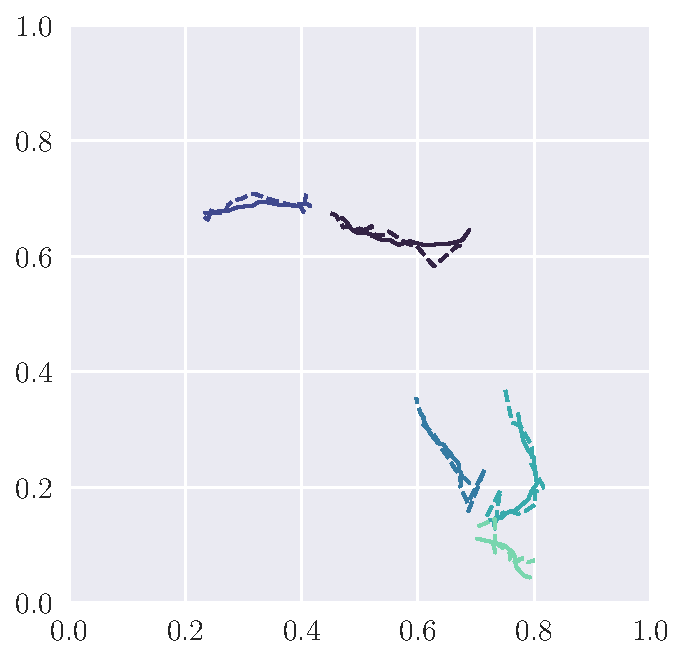
\includegraphics[width=\linewidth]{project/latex/figures/test_model.pdf}
    \caption{Predicted trajectories in dashed lines, and labels in full lines. 5 different sequences, consisting of 19 time steps.}
    \label{fig:test_model}
\end{figure}


%================================================================
\section{Future work}\label{sec:future_work}
%================================================================
Next step is to set up an experiment using both train and test set, where I collect data during both training and testing. I will also investigate different parameters such as learning rate and optimizers. In addition, I will compare the model performance using simulated and experimental data, using Sargollini data.
% %================================================================
\section{Protocol}\label{sec:protocol}
%================================================================
\begin{description}
    \item[29.02.24] Decided on main article to base the project on \cite{sorscher:2023:unified_theory} with support from \cite{banino:2018:vector_based}. Set up a conda environment for the project, which included \verb|PyTorch| and \verb|RatInABox| \cite{george:2022:ratinabox}. Produced a test trajectory, found out how to export the velocity and position data and convert to tensor. Started the implementation of vanilla RNN class.
    
    To do:
    \begin{enumerate}
        \item Read the chapter on RNN in GBC.
        \item Need to figure out how to generate multiple trajectories and build a multi-dimensional tensor.
        \item Also, how to take the velocity data as input in batches of sequences. 
    \end{enumerate}

    \item[01.03.24] Went over a general setup of RNNs using \verb|PyTorch|, and set up a vanilla RNN. Howerver, I'm having issues with the dimensions of the data and the layers so it is not working. Read chapter 10.1-10.6 and 10.12 in GBC \cite{gbc:2016:deep_learning} about RNNs.

    To do:
    \begin{enumerate}
        \item Read chapter 10.7-10.11 in GBC.
        \item Still, figure out how to generate multiple trajectories and which format to save in.
        \item Also, how to take the velocity data as input sequences with correct dimensions of input and layers.
        \item Is it necessary to build a multi-dimensional tensor and use embedding?
    \end{enumerate}

    \item[04.03.24] Read chapter 10.7-10.11 in GBC, the mathematical basis for RNNs is relevant in understanding how it is built using module in PyTorch. Read the paper from Xu et. al. \cite{xu:2022:conformal}, where they study conformal isometry in a model based on a continuous attractor neural network. They focused on a RNN that represented the self-position linearly and the input velocity additively, they also included ReLU. Noted down equations and thoughts in Goodnotes notebook, to get a better understanding of their implementation. In addition, I went through a couple of the papers refered to, and their github repos (Gao \cite{gao:2019:learning_gridlike, gao:2021:path_integration} and Banino \cite{banino:2018:vector_based}). 

    List of repos:
    \begin{description}
        \item[Gao]  \url{https://github.com/ruiqigao/GridCell}
        \item[Gao] \url{https://github.com/ruiqigao/grid-cell-path}
        \item[Xu] \url{https://github.com/DehongXu/grid-cell-rnn}
        \item[Sorscher] \url{https://github.com/ganguli-lab/grid-pattern-formation}
        \item[Banino] \url{https://github.com/google-deepmind/grid-cells}
        \item[RatInABox] \url{https://github.com/RatInABox-Lab/RatInABox}
    \end{description}
    
    To do:
    \begin{enumerate}
        \item Generate multiple trajectories using \verb|RatInABox|, and save in batches of trajectories. Look into the Sorscher implementation, as they use PyTorch (batch\_size, sequence\_length, input\_size). 
        \item The velocity data are input sequences, figure out correct dimensions of input and if it necessary to include encoder/decoder layers.
    \end{enumerate}

    \item[06.03.24] Meeting with Markus, to go over plan for thesis. Fixed the thesis document and put in the main section titles for the neuro background. Started with the computational background. Both sections which can be used in this project, maybe in lesser detail.

    To do: %
    \begin{enumerate}
        \item Fix code!
    \end{enumerate}

    \item[07.03.24] Wrote function for generating trajectories, and figured out how to put the position and velocity into a tensor and save to file.

    To do: %
    \begin{enumerate}
        \item Figure out dataloader in PyTorch.
        \item Start implementing RNN.
    \end{enumerate}

    \item[12.03.24] Wrote a draft introduction, including both an artificial and a biological perspective on neuroscience. Found relevant background on brain anatomy in the neuroscience textbook \cite{bear:2016:neuroscience}, in addition to some detailed theory in the book about learning and memory \cite{byrne:2008:learning_memory}. I have also set up a basic rnn using only a torch.rnn and a decoder. The code runs, however, it does not predict the correct path...! 

    To do: %
    \begin{enumerate}
        \item Build a model using the Module class provided by PyTorch.
        \item Test different parameters, optimizers etc.
        \item Customize the environment of the agent, maybe insert rewards etc.
    \end{enumerate}

    \item[14.03.24] Built VanillaRNN using the Module class. it runs, however, it does not initiate a hidden state before running. 

    To do: %
    \begin{enumerate}
        \item Fix initial hidden state.
        \item Test different parameters, optimizers etc.
        \item Customize the environment of the agent, maybe insert rewards etc.
    \end{enumerate}

    \item[15.03.24] Fixed the initiation of the hidden state, and the model now makes similar trajectory predictions. Need to shift the label (position) array one time step when computing loss and comparing paths.

    To do: %
    \begin{enumerate}
        \item Account for the difference in time, since the predicted position is one time step ahead of the label.
        \item Test different parameters, optimizers etc. to see if it is possible to decrease loss. 
        \item Customize the environment of the agent, could be interesting to insert objects and see it the agent can learn how to navigate the environment and recognize objects after retention.
    \end{enumerate}

    \item[18.03.24] Cleaned up the code and put it into scripts, fixed the time step difference when computing loss. Also added a plot showing the current model predictions for 5 trajectories. Fixed report setup, still needs proofreading and some more details in both the introduction and the progress report.

    To do: %
    \begin{enumerate}
        \item Finish report!
        \item Test different parameters, optimizers etc. to see if it is possible to decrease loss. 
        \item Customize the environment of the agent, could be interesting to insert objects and see it the agent can learn how to navigate the environment and recognize objects after retention.
    \end{enumerate}

    \item[08.04.24] Finish draft of introduction, and set up the structure of the theory section using keywords. Added a few articles on theory and method related subjects into reference section.

    To do: %
    \begin{enumerate}
        \item Fix training method, separate into forward and predict and include a separate method for training. 
        \item Set up new model where head direction is added as input, in addition to velocity. Compare both model accuracy.
        \item Experiment with different parameters, such as learning rate and schedulers.
        \item Write theory section, include biological and artificial background.
    \end{enumerate}

    \item[22.04.24] Finish the vanilla RNN and implemented a separate train method, write new main method to use new training scheme.

    To do: %
    \begin{enumerate}
        \item Set up new model where head direction is added as input, in addition to velocity. Compare both model accuracy.
        \item Experiment with different parameters, such as learning rate and schedulers.
        \item Start writing the report!
    \end{enumerate}

    \item[23.04.24] Adjusted some of the parameters to see if it affected the computation and prediction. When increasing number of hidden neurons the model seems more prone to gradient explosion, as the loss increase drastically. Also, tried to increase number of trajectories generated, and number of epochs.

    \begin{enumerate}
        \item Set up new model where head direction is added as input, in addition to velocity. Compare both model accuracy.
        \item Write up the theory section for both the biology and machine learning part. None of these sections need to be mathematically detailed, as this will be put in the methods section.
    \end{enumerate}

    \item[01.05.24] Started to write on the theory and method sections, but I'm struggling to put all the information I want to include in order. Should try to put it into a mind map to see if I can find the red thread or something.

    What I want is for the introduction to set the stage, I should mention some background here to ground the project in. I also have to present the layout of the report. 

    In the theory section I want to delve a bit deeper into what is presented in the introduction, such as previous experiments of rats performing spatial tasks and the importance of hippocampus in those tasks. For the machine learning part I want say something about the advantage of using computational tools in neuroscience, and some background for previous work using neural networks in the study of place cells etc.

    In the method section I will present any mathematical stuff related to the machine learning stuff, in addition to algorithms. I want to start out by presenting the basic feed forward neural networks, and move on to include recurrent neural networks for the time sequence data. If time allows I want to include something generative, the methods for this I'll include if necessary. I need to include a tool section and maybe a separate section for generating data, and mention what type of setup and data I produce and maybe why?

    The result section should be pretty straight forward, start with the default environment to build the model an make predictions. Tweek the model to see if I can lower the loss? Continue with comparing the model's performance on experimental data. If time allows, include objects and possibly generate trajectories based on learned location (learn short cut).

    Discuss and conclude the findings, suggest any future work.

    \item[21.05.24] Cleaned up the function for creating dataset and put it into a utils module, separated into subfunction to either import Sargolini data or generating synthetic trajectories. Main function control whether the data is saved or not. 

    Next up:
    \begin{enumerate}
        \item Write function to include other features when creating dataset, such as head-direction.
        \item Figure out the size and shape of the environment used in the Sargolini data.
        \item Figure out the argparser and dataclass.
    \end{enumerate}

    \item[22.05.24] Cleaned up the model and implemented use of parser.

    Next up:
    \begin{enumerate}
        \item Have a look at the generated dataset, fix the number of trajectories so that it can be more than batch size!
        \item Implement the option to include other features when creating dataset, such as head-direction.
        \item Figure out the size and shape of the environment used in the Sargolini data.
    \end{enumerate}

    \item[23.05.24] Fixed the function for generating synthetic data, it now creates dataset of a given number of trajectories instead of batch size. The size of the square boxes used in Sargolini are 
    \begin{itemize}
        \item a small square box (100 × 100 × 50 cm high; aluminium)
        \item a large square box (150 x 150 x 50 cm high; polyethylene)
    \end{itemize} 
    % Today: implement model that takes in head direction, and adapt the data generator to add this as well. Maybe add some more hidden layers to the model, and split into rnn and connectivity layers?

    Next up:
    \begin{enumerate}
        \item Figure out which of the Sargolini data is used, to determine box size.
        \item Separate the full trajectory into smaller with the correct sequence length.
    \end{enumerate}

    \item[24.05.24] Fixed the model so that it can take in any number of inputs. The issue kind of lies in how the data is generated, and I have to fix the generator function.

    \item[27.05.24] Started cleaning up the project, consider using class to create and handle the dataset. Found some info on how to do this at \url{https://medium.com/analytics-vidhya/pytorch-for-deep-learning-feed-forward-neural-network-d24f5870c18}. Order of writing the report is going to be:
    \begin{enumerate}
        \item Theory, including hypothesis \footnote{Hypothesis: Does the path of an animal rely on the animals previous steps (FFNN vs. RNN), is the loss affected by how many time steps are included (length of trajectory), will more input features increase the precision of the prediction(vel, head ++). Additional: can an increase in hidden layers in the network act similarly as the layers in MEC and hippocampus?}
        
        \item Methods, starting with the data generation. Add the equations for the models, FFNN and especially RNN, and any algo for training and assessing (backprop, optim, learning rate ++). Also add a section on testing, as well as tools used.
        
        \item Result and discussion, going in order of implementation (follow development of hypothesis).

        \item Introduction, lay out the motivation for the project with a background in neurobiology. 

        \item Conclusion, wrap it up and add a paragraph on possible future work.

        \item Abstract, the condensed thingy.

        \item Appendix and references, make sure everything is in order!
    \end{enumerate}

    In addition to the report, I have to make sure the code is working and looks good. Finish up by cleaning up the repo, add doc strings and unit tests, and write up the readme with instructions on how to run the code.
\end{description}
% % Background
Hippocampus important in spatial representation and memory, and self position may be stored here - how?
Grid cells signal the change in position, and position is integrated where?
If grid cells path integrate based on speed and direction, where is the sensory cues processed?
% Used info from the article \cite{moser:2008:spatial_representation}
% For path integration use Banino et al as main

% Questions
Set up a network (rnn) which path integrates based on input such as velocity, head direction etc. Move on to maze, insert objects and have the network identify these objects based on position, or even find its way out based on spatial cues?
- How to set up network with object recognition, how is the information about the object used as input?
- If the networks output is a position, is this position matched with information in a mazemap? 
- Want to use visual and locomotion cues as input in navigation tasks

% Aim 
- Set up network to perform path integration based on velocity, compare performance using synthetic data and experimental data. 
- Include other cues such as head direction and visual cues, when determining position.
- Include objects and object recognition, consider using several networks and have path integration done by rnn then integrate with visual cues?
- Generate path based on task of finding object?


%==================== Abstract ===============================================
% A quick overview of what has been done, and the most important results, 
% consise and to the point.
%=============================================================================
To do!


%==================== Introduction ===========================================
% Motivate the reader and present overarching ideas, and background on the 
% subject of the project. Mention what I have done and present the structure 
% of the report, that is how it is organized.
%=============================================================================
The human brain is an extraordinary computer. It processes huge amounts of data during one day, which allow us to interact with and react to our surroundings. % https://www.britannica.com/science/information-theory/Physiology 
One fascinating feature is the ability to navigate and store memories, and a region important in spatial navigation and memory is the medial temporal lobe, where the entorhinal-hippocampal circuit lies. Early research found that lesions in the hippocampal area impaired the rat's ability to navigate %(Morris, R., Garrud, P., Rawlins, J. et al. Place navigation impaired in rats with hippocampal lesions. Nature 297, 681–683 (1982). https://doi.org/10.1038/297681a0) 
and taxi drivers who suffered stroke, damaging the hippocampus, could no longer recall trajectories \cite{maguire:2000:navigation}.

Recent studies have found that information on self position is computed in upstream from the hippocampus, and that the hippocampus itself is important in memory formation.

It is common to use model animals in research related to the human brain, as the ethical aspect of invasive methods make it difficult to use human as a model. In neuroscience, machine learning has become a useful tool, as it allows us to investigate several hypotheses, before testing the the most promising ones in animal models. This process can speed up the time of testing, while reducing the number of animal lives sacrificed.

Episodic memory is a type of declarative memory, which includes the ability to recall previous experiences. These memories include the element of what, when and where.

\textbf{Draft introduction}
In neuroscience, machine learning has become a useful tool, as it can ie. reduce dimensionality in data \cite{Badrulhisham:2024:ml_and_ai_in_neuroscience}. It allows us to investigate several hypotheses, before testing the the most promising ones in animal models. This process can speed up the time of testing, while reducing the number of animal lives sacrificed. 

One machine learning method is artificial neural network. It was inspired by the synapses in the brain, and has been found useful in neuroscience. 
% Add more on machine learning
One interesting circuit to investigate, is the entorhinal-hippocampal circuit, which is thought to be vital in navigation \cite{okeefe:1978:hippocampus, hafting:2005:microstructure}. Using biological plausible conditions, the neural network can learn how to path integrate \cite{banino:2018:vector_based}.

The aim of this project is to train a neural network to learn trajectories, using velocity data as input. Since the trajectories are time dependent, and the model take sequential data as input, I will implement the model using a recurrent neural network. In addition, I will use increase input and use both velocity and head direction, and compare the predicted trajectories.

First, I will present a theoretical background for the project in section \ref{sec:theory}. I will give a brief overview of the relevant neurobiological circuits, and artificial neural networks, before presenting the methods used in implementing the models in section \ref{sec:methods}. In section \ref{sec:results} I present the result, followed by a discussion in section \ref{sec:discussion}. Lastly, I conclude my findings in section \ref{sec:conclusion}, and include possible future research questions.

% The goal of basic research in neuroscience, is to understand how the brain works. As the brain is made up of three main parts - the cerebrum, cerebellum and brainstem. Many advances have been made, based on people suffering from injuries. Such as Phineas Gage who survived an iron rod through his skull, which damaged his frontal lobe. A change in Gage's behavior led scientists to understand the function of the frontal lobe in humans...

% Throughout history, several psychiatric treatments have been important in understanding the human brain. However, knowing the function of the main areas of the brain, is not enough in understanding the brain as a whole. Moving down to a molecular level, we still have a lot to learn. 

% Basic research in neuroscience aims to further understand of the human brain. In knowing the baseline we can more easily understand the mechanisms affected in a diseased brain, what happens to the healthy brain when an individual gets Alzheimer disease or a stroke damages the brain tissue. 

% In the hunt for answers it is common to use model organisms, and with increasing complexity of the research question it is often necessary to use mammals in order to study the behavior in both wild type and variants. However, in order to reach a point in the research where an animal experiment is both possible and necessary to further the understanding, we have to have a plausible hypothesis to test. 

The human brain is an extraordinary computer. It processes huge amounts of data during one day, which allow us to interact with and react to our surroundings. % https://www.britannica.com/science/information-theory/Physiology 
One fascinating feature is the ability to navigate and store memories, and a region important in spatial navigation and memory is the medial temporal lobe, where the entorhinal-hippocampal circuit lies. Early research found that lesions in the hippocampal area impaired the rat's ability to navigate %(Morris, R., Garrud, P., Rawlins, J. et al. Place navigation impaired in rats with hippocampal lesions. Nature 297, 681–683 (1982). https://doi.org/10.1038/297681a0) 
and taxi drivers who suffered stroke, damaging the hippocampus, could no longer recall trajectories \cite{maguire:2000:navigation}.

Recent studies have found that information on self position is computed in upstream from the hippocampus, and that the hippocampus itself is important in memory formation.

It is common to use model animals in research related to the human brain, as the ethical aspect of invasive methods make it difficult to use human as a model. In neuroscience, machine learning has become a useful tool, as it allows us to investigate several hypotheses, before testing the the most promising ones in animal models. This process can speed up the time of testing, while reducing the number of animal lives sacrificed.

Episodic memory is a type of declarative memory, which includes the ability to recall previous experiences. These memories include the element of what, when and where, 


%=================================== Theory ==================================
In the theory section I want to delve a bit deeper into what is presented in 
the introduction, such as previous experiments of rats performing spatial 
tasks and the importance of hippocampus in those tasks. For the machine 
learning part I want say something about the advantage of using computational 
tools in neuroscience, and some background for previous work using neural 
networks in the study of place cells etc.
\begin{itemize}
    \item Anatomy: Hippocampus and its connected areas, in formation and recall of memory.
    \item Function: Spatial memory formation
    \item Methods: In vivo, including model animals and human
    \item Alternative: How scientific discoveries were made which led to a basic understanding of the human brain, and how ethics make this way of doing research problematic. In comes machine learning!
\end{itemize}
%=============================================================================
When we experience something new, the memory we form depend on the elements what, when, and where. An episodic memory links all these elements into one event, like your first time riding a bicycle. You can likely recall the color of your bike, what season it was, and the street you rode in. Especially if you fell of the bike and hit yourself, which would have resulted in an emotional link to the memory.

The hippocampus is important in forming new episodic memories. This was discovered when the patient known as H.M. had both hippocampi surgically removed to stop the seizures, and was not able to form any new memories \cite{scoville:1957:loss_recent}. In studies done with rats, hippocampal lesions\footnote{Lesion information} resulted in poor performance in navigation tasks \cite{kaada:1961:maze, schlesiger:2013:hippocampal_activation_maze}. 

How is the hippocampus important in spatial memory? Positional information is seen in so-called place cells, from recordings in rats. These neurons are thought to encode a spatial map of the environment \cite{okeefe:1978:hippocampus}. The hippocampus receives input from the association cortex, which is where the entorhinal cortex lies. The activity recorded in the entorhinal cortex form similar pattern as seen in place cells. However, the pattern is repetitive and the size differs between layers, forming grid patterns \cite{hafting:2005:microstructure}. These neurons are called grid cells. In addition, neurons encoding the direction of the rats head...

When the rat performs a task such as running on a track, recording neuron activity in the hippocampus result in place fields. These can be ordered according to the rats position when the neuron fired, which result in a sequence of active neurons depending on time.

Recent studies have applied machine learning methods, to understand the connection between grid cells and place cells in navigation \cite{banino:2018:vector_based}. The use of deep neural networks in neuroscience, have made it possible to test hypotheses using biologically plausible conditions. 

% The entorhinal-hippocampal circuit has been found important in how mammals navigate in space. Focus on hippocampus and spatial memory in navigation, as the hippocampus receives information from all sensory modalities.

% Discoveries as to how the brain works where often made when people suffering from brain injuries showed a change in behavior. One such discovery was with the patient abbreviates as H.M. who ... removed hippocampi. His declarative memory was affected, as he could not form any new memories.

% In rats, bilateral removal of hippocampus resulted affected their ability to perform in maze experiments \cite{kaada:1961:maze}.

%==================== Methods ===============================================
% Describe the methods and algorithms used, include any formulas. Explain how 
% everything is implemented, and possibly mention the structure of the 
% algorithm. Add demonstrations such as tests, selected runs and validations. 
%============================================================================
RatInABox

% ANN
The artificial neural network (ANN) was first described by Warren McCulloch and Warren Pitts, by signal processing in the brain using an abstract approach \cite{mcculloch:1943:logical}. In recent years, neural networks have shown many use cases and have evolved into several types of networks.

A general neural network consist of layers of neurons. The output of one neuron can be described as 
\begin{equation}
    y = f \bigg( \sum_{i=1}^{n} w_{i} x_{i} + b_{i} \bigg) = f(z),
\end{equation}
where $f$ is a non-linear activation function and $n$ is the number of inputs received. 
% In matrix-vector form: h = g(W^{T} x + b)

% FFNN
In the feed-forward neural network (FFNN), the information moves through the layers in one direction. The network is said to be fully connected if each neuron in a layer is connected to all neurons in the next layer. Figure ... illustrates a FFNN, with one input layer, one hidden layer, and one output layer. 


% RNN
When dealing with sequential data, a standard FFNN is not able to ensure the ordering of the data. To account for the dependency between the input data, we can use a recurrent neural network (RNN). The network has recurrent connections between the hidden neurons, and produce an output at every time step. In a vanilla RNN, the output from a hidden layer at time step $t$ can be written as 
\begin{equation}
    \mathbf{h}^{(t)} = f \bigg( \mathbf{Wh}^{(t-1)} + \mathbf{Ux}^{(t)} +  \mathbf{b} \bigg), 
\end{equation}
where $\mathbf{W}$ and $\mathbf{U}$ are weight matrices, $\mathbf{b}$ is a bias vector, $\mathbf{h}$ is the recurrent state vector, and $\mathbf{x}$ is the input vector.

%% Activation function
To generate output from a neuron the input is transformed using a non-linear activation function, which is determined by the nature of the data. In neuro it is common to use the ReLU function in the hidden neurons, as it emphasizes the need for an input to reach a threshold to fire.

%% Loss function 
Using MSE to determine cartesian coordinates in the output layer.

%% Backpropagation
Whe


%% Decoding the firing using rate maps
Since the aim is to model place cells during path integration, it is necessary to decode the firing pattern to validate the performance. 

To simulate the exploratory behavior and movement of rats I generated trajectories using the package RatInABox \cite{george:2022:ratinabox}. It also allowed me to import the experimental data from Sargolini et al \cite{sargolini:2006:conjunctive} to compare with.

Tools

\textbf{Draft methods}
\subsection{Feed forward neural network}\label{sssec:ffnn}
The artificial neural network (ANN) can be compared with the neural network of the brain. Each neuron in the ANN receives a signal which is processed and result in an output if the signal reaches a given threshold. The signal is determined by the connectivity in the ANN, the threshold by the activation function, and the data processing moves in one direction making it a feed forward neural network (FFNN).
% Rewrite to move FFNN info into the first sentence, after introducing ANN
% Mention general architecture, including input layer, hidden layers and output layer, as well as activation function, loss function, update of weights and bias using gradient based approach.
A general feed forward neural network consist of an input layer, a number of hidden layers, and an output layer. Each layer consist of nodes, or neurons, where values are determined by an activation function given by 
\begin{align}
    y = f \bigg( \sum_{i=1}^{n} w_{i} x_{i} + b_{i} \bigg) \ .
\end{align}

When training the network, it is necessary to compute the error of the prediction and have the network learn from the error. To do this it is common to use the backpropagation algorithm, which computes the gradient of 

\subsection{Recurrent neural network}\label{sssec:rnn}
When doing path integration, the next step in the trajectory will depend on the previous step. A FFNN does not account for the time dependency, introducing the recurrent neural network (RNN). The RNN is best suited for sequential data, where each element of feature have to occur in a given order. In the case of a rats path in exploring an environment (explain dead reckoning) the rat need to know where it has been to be able to get back to its original position. To set this up in a neural network, each layer will receive an input (velocity) in addition to the recurrent state from previous step.

% \subsection{Generative models}\label{sssec:generative}

\subsection{Tools}\label{sssec:tools}
The RNN is implemented in \verb|Python|, using \verb|PyTorch| to build the models. The trajectory data is generated using \verb|RatInABox|. I use the library \verb|matplotlib| to produce all figures, and stylize them using \verb|seaborn|. 

\subsection{Data}\label{sssec:data}
Synthetic data, default two dimensional environment with an agent moving. Sample velocity and positions of the agent, other data such as head direction etc. is possible to increase number of features.

To simulate the exploratory behavior and movement of rats I generated trajectories using the package RatInABox \cite{george:2022:ratinabox}. It also allowed me to import the experimental data from Sargolini et al \cite{sargolini:2006:conjunctive} to compare with.


%==================== Results and Discussion ================================
% Present results and give a critical discussion of my work in the context of 
% other work. Relate the work to previous studies, and make sure the results 
% are reproducible. Include information in figure captions such that they can 
% give the reader enough to understand the main gist of the report.
%============================================================================



%==================== Conclusions and Perspectives ==========================
% State main findings and interpretations, as well as a perspective on what 
% can be done in future work. Discuss any pros and cons of the methods used, 
% and include any possible improvements.
%============================================================================
 
%-------- bibliography ----------- 
\newpage 
\bibliography{references}

%-------- appendix -----------
% \newpage
% \onecolumngrid
% \appendix
% \input{sections/appendix}

%-------- Structure -----------
% \tableofcontents 

\end{document}
%==========================================================
% ------------------- end of main content ---------------
%==========================================================